\documentclass[11pt]{article}

\usepackage[a4paper, total={16cm, 24cm}]{geometry}
\usepackage[portuguese]{babel}
\usepackage[utf8]{inputenc}
\usepackage{graphicx}
\usepackage{amsmath}
\usepackage{tikz}
    \usetikzlibrary{shadows}
\usepackage{booktabs}
\usepackage[colorlinks=true]{hyperref}
\usepackage{listings}
    \renewcommand\lstlistingname{Listagem}
    \lstset{numbers=left, numberstyle=\tiny, numbersep=5pt, basicstyle=\footnotesize\ttfamily, frame=tb,rulesepcolor=\color{gray}, breaklines=true}
\usepackage{blindtext}
\usepackage[export]{adjustbox}

% -------------------------------------------------------------------------------------------
\title
{
    
\includegraphics[width=0.4\textwidth]{imgs/university.png}
    \\[0.1cm]
    \textbf{3º Trabalho - Mazy Luck} \\
    Estrutura de Dados e Algoritmos II
}

\author
{
    \textbf{Professora:} Vasco Pedro \\
    \textbf{Realizado por:} Filipe Alfaiate (43315), Miguel de Carvalho (43108)
    \textbf{Grupo:} g308
}
\date{\today}

% -------------------------------------------------------------------------------------------
%                                Body                                                       %
% -------------------------------------------------------------------------------------------

\begin{document}
\maketitle

% -------------------------------------------------------------------------------------------
\section{Algoritmo}

\hspace{0,6cm}O nosso algoritmo consiste na utilização de um \textbf{grafo orientado cíclico
com pesos}, pertencentes aos \textbf{números inteiros}. O grafo contém \textbf{vértices}, que
representam as \textbf{salas}, e \textbf{arcos}, que representam os \textbf{corredores entre
as salas}.

Cada \textbf{sala} contém o \textbf{identificador da sala}, a \textbf{distância} a que ela se 
encontra da sala inicial e a \textbf{sala que a precede}. 

Cada \textbf{corredor} contém duas salas, a \textbf{sala de origem} e a \textbf{sala de destino},
e um \textbf{custo} para o poder atravessar. O \textbf{custo é positivo} quando se encontra um
\textbf{saco} com uma certa quantia de dinheiro e \textbf{é negativo} quando se encontra um
\textbf{crocodilo}, sendo necessário gastar uma certa quantia para baixar a ponte e atravessar o
corredor em segurança, essa quantia é descontada em \textbf{débito} ou em \textbf{crédito}.

A utilização deste algoritmo baseia-se no caminho mais curto (apresenta um menor custo) desda
\textbf{sala inicial} até à \textbf{sala final}, obtendo como resultado a possibilidade do
Dirk \textbf{perder dinheiro ao percorrer o labirinto}.

% -------------------------------------------------------------------------------------------
\section{Análise do Grafo}

\hspace{0,45cm} Tendo o labirinto pronto a ser percorrido, colocamos a distância da \textbf{sala 
inicial} a zero. 

Em seguida, percorremos todos os \textbf{corredores} o mesmo número de vezes quanto as salas existentes no
labirinto. Para cada corredor verificamos se a \textbf{sala de origem} tem uma distância conhecida,
caso apresente, somamos a distância com o custo do corredor, comparando se o resultado é menor que a
distância entre a \textbf{sala inicial} e a \textbf{sala de destino}, caso se verifique a condição
a \textbf{sala de destino} fica com o resultado da soma e um precedente que é a sala de origem.
Com o término desta pesquisa percorremos todos os corredores uma última vez para verificar se 
existe um \textbf{ciclo} cujo o saldo ao percorrer o mesmo é negativo, ou seja, ganha 3 quantias
e perde 6, logo tem um saldo negativo de 3.

\newpage
Segue-se uma ilustração do problema:

\begin{figure}[h!]
    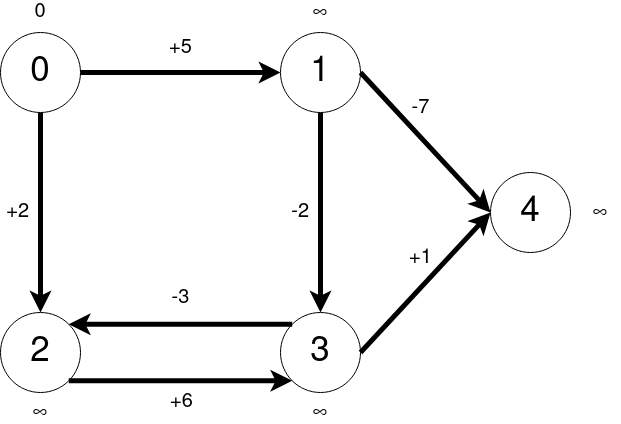
\includegraphics[width=0.55\textwidth, center]{imgs/grafo1.png}
    \caption{Labirinto inicial}
    \label{fig:grafo1}
\end{figure}

\begin{figure}[h!]
    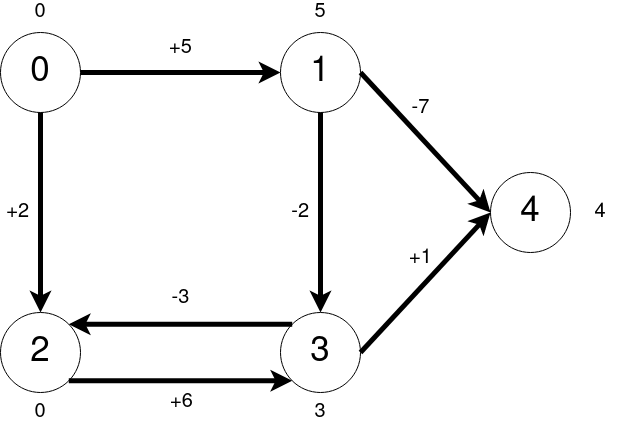
\includegraphics[width=0.55\textwidth, center]{imgs/grafo2.png}
    \caption{Labirinto com a distância mais curta desde o vértice 0 até aos outros}
    \label{fig:grafo2}
\end{figure}

\begin{figure}[h!]
    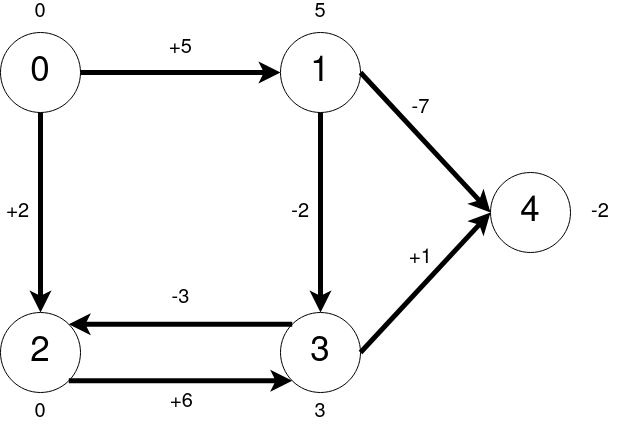
\includegraphics[width=0.55\textwidth, center]{imgs/grafo3.png}
    \caption{Labirinto com o caminho mais curto para todos os vértices com origem no vértice 0}
    \label{fig:grafo3}
\end{figure}
\newpage
% -------------------------------------------------------------------------------------------
\section{Complexidade}
\subsection{Temporal}

\hspace{0,5cm}Começámos por proceder à leitura de uma \verb|string| com 2 números, \textbf{número
de salas}, \textbf{número de corredores}, respetivamente, o que origina uma complexidade constante
\verb|O(1)|.

\begin{center}
    \textbf{O(1) = O(1)}
\end{center}

De seguida criámos dois vetores para representar todas as salas e todos os corredores, que apresenta
um custo constante \verb|O(1)|.

\begin{center}
    \textbf{O(1) = O(1)}
\end{center}

Posteriormente procedemos à leitura do resto das linhas de input com um ciclo com um número
de iterações igual ao número de corredores, que apresenta, 3 números e uma letra, \textbf{sala
de origem}, \textbf{sala de destino}, a representação de um número positivo ou negativo (
\textbf{B} ou \textbf{C}) e o \textbf{custo}. Tanto a leitura de input, as afetações realizadas
e a condição apresentam um custo constante \verb|O(1)|.

Ainda dentro do mesmo ciclo, após a afetação do input às variáveis correspondentes, verificou-se
se a \textbf{sala de origem e de destino} existem, caso não existam são criadas com um número e
uma distância que representa o infinito, colocando-as num vetor de salas, ou seja, apresenta um
custo constante \verb|O(1)|. Para além da verificação da existência de sala é criado também um
corredor com o custo, a \textbf{sala de origem} e a \textbf{sala de destino}, colocando-o no 
vetor de todos os corredores. Tal como as afetações realizadas acima, esta também tem custo
constante \verb|O(1)|.

\begin{center}
    \textbf{O(1) + O(1) + O(1) = O(1)}
\end{center}

Com o término da leitura dos inputs podemos afirmar que tem uma complexidade linear \verb|O(E)|,
onde \verb|E| é o número de corredores do labirinto.

\begin{center}
    \textbf{O(1) x O(E) = O(E)}
\end{center}

Afetámos a distância da \textbf{sala inicial}, o que origina um custo constante \verb|O(1)|.

\begin{center}
    \textbf{O(1) = O(1)}
\end{center}

Com tudo preparado para realizar o algoritmo \textbf{Bellman-Ford} procedeu-se à sua execução.
Nessa execução irão ser realizados dois ciclos, onde o ciclo exterior percorre todas as \textbf{salas}
e o interior todos os \textbf{corredores}. A cada iteração do ciclo interior serão realizadas
condições, afetações e operações todas com uma complexidade constante \verb|O(1)|, originando uma
complexidade \verb|O(VE)|, onde \verb|V| é o número de \textbf{salas} do
labirinto e \verb|E| é o número de \textbf{corredores} do labirinto.

\begin{center}
    \textbf{O(1) + O(V) x O(E) = O(VE)}
\end{center}

Por fim, percorremos uma última vez todos os \textbf{corredores} verificando se existe algum caminho
mais curto, obtendo uma complexidade \verb|O(E)|, onde \verb|E| é o número de \textbf{corredores}.

\begin{center}
    \textbf{O(E) = O(E)}
\end{center}

Complexidade final:

\begin{center}
    \textbf{O(1) + O(1) + O(E) + O(1) + O(VE) + O(E) = O(VE)}
\end{center}

\subsection{Espacial}

\hspace{0,5cm} Para ler os inputs é necessário criar um array de strings onde o seu tamanho
varia consoante o número de palavras lidas durante a inserção do input, ocupando assim $\theta(L)$,
onde \verb|L| é o número de elementos lidos entre espaços.

Todas as variáveis do \textbf{tipo inteiro} terão uma ocupação em memória constante \verb|O(1)|.

Durante a inicialização dos vetores terão de ser reservados espaços na memória,
um com tamanho \verb|V|, que ocupa em memória \verb|O(V)|, onde \verb|V| é o número de
\textbf{salas} do labirinto, e outro com tamanho \verb|E|, que ocupa em memória \verb|O(E)|,
onde \verb|E| é o número de \textbf{corredores} do labirinto.

Na execução do ciclo onde lê o resto dos inputs é criado um array de strings onde o seu tamanho
varia consoante o número de palavras lidas durante a inserção do input, ocupando assim $\theta(L)$,
onde \verb|L| é o número de elementos lidos entre espaços. Como em cada ciclo cria um novo array
a complexidade espacial multiplica pelo número de corredores, tendo então uma complexidade de
\verb|O(EL)|, onde \verb|E| é o número de corredores.

Ainda no mesmo ciclo, são criados \textbf{salas} e \textbf{corredores} onde as \textbf{salas} e os
\textbf{corredores} terão uma complexidade \verb|O(1)|. 
% -------------------------------------------------------------------------------------------
\section{Comentários Adicionais}

\hspace{0,5cm}No decorrer do projeto existiram diversas fases de desenvolvimento, uma fase 
de entendimento, uma fase de pesquisas e dúvidas, uma fase de desenvolvimento do trabalho e
uma última fase de debug.

Nesta última fase deparámos-nos com um problema que permitiu evoluir
o nosso conhecimento. Quando somado o maior número inteiro de 32 bits com outro número natural
é criado um overflow, isto significa que os 32 bits não são suficientes para representar esta
soma. Como solução o processador, para continuar a executar corretamente o programa, coloca
todos os bits a zero e continua a somar o restante a partir desse ponto, originando um número
errado. Para solucionar este problema bastou apenas fazer uma verificação, onde é
verificado se a distância da respetiva sala é igual ao número inteiro máximo de 32 bits. 
% -------------------------------------------------------------------------------------------
\end{document}